\section{What is artificial intelligence?}
\setauthor{Romeo Bhuiyan}
The concept of AI has a long history that dates back to ancient times, when people first tried to build machines that could mimic human abilities. In the modern era, the term "AI" was first coined in 1956 by computer scientist John McCarthy, who defined it as "the science and engineering of making intelligent machines."
\\
\\
These machines are designed to be able to perform tasks that typically require human intelligence, such as visual perception, speech recognition, decision-making, and understanding natural language. AI can be applied to a wide range of fields, from healthcare and finance to education and transportation, with the goal of making systems more efficient and effective. AI can be classified into two broad categories: narrow or weak AI, which is designed to perform a specific task, and general or strong AI, which has the ability to perform any intellectual task that a human being can perform.

\section{Philosophy of artificial intelligence}
\setauthor{Christioph Lasinger}

\section{The future of artificial intelligence}
\setauthor{Romeo Bhuiyan}

\section{How does a neural network work?}
\setauthor{Romeo Bhuiyan}
A neural network is a type of machine learning algorithm modeled after the structure and function of a human brain (neural linking). It is composed of many interconnected processing nodes, called neurons, which work together to process information. 
\\
\\
Each neuron receives input from other neurons, processes that information, and produces an output. This output is then passed on to other neurons in the next layer of the network. In this way, information is passed through the network, from the input layer to the output layer, allowing the neural network to learn and make predictions based on the data it is given.
\\
\\
\\
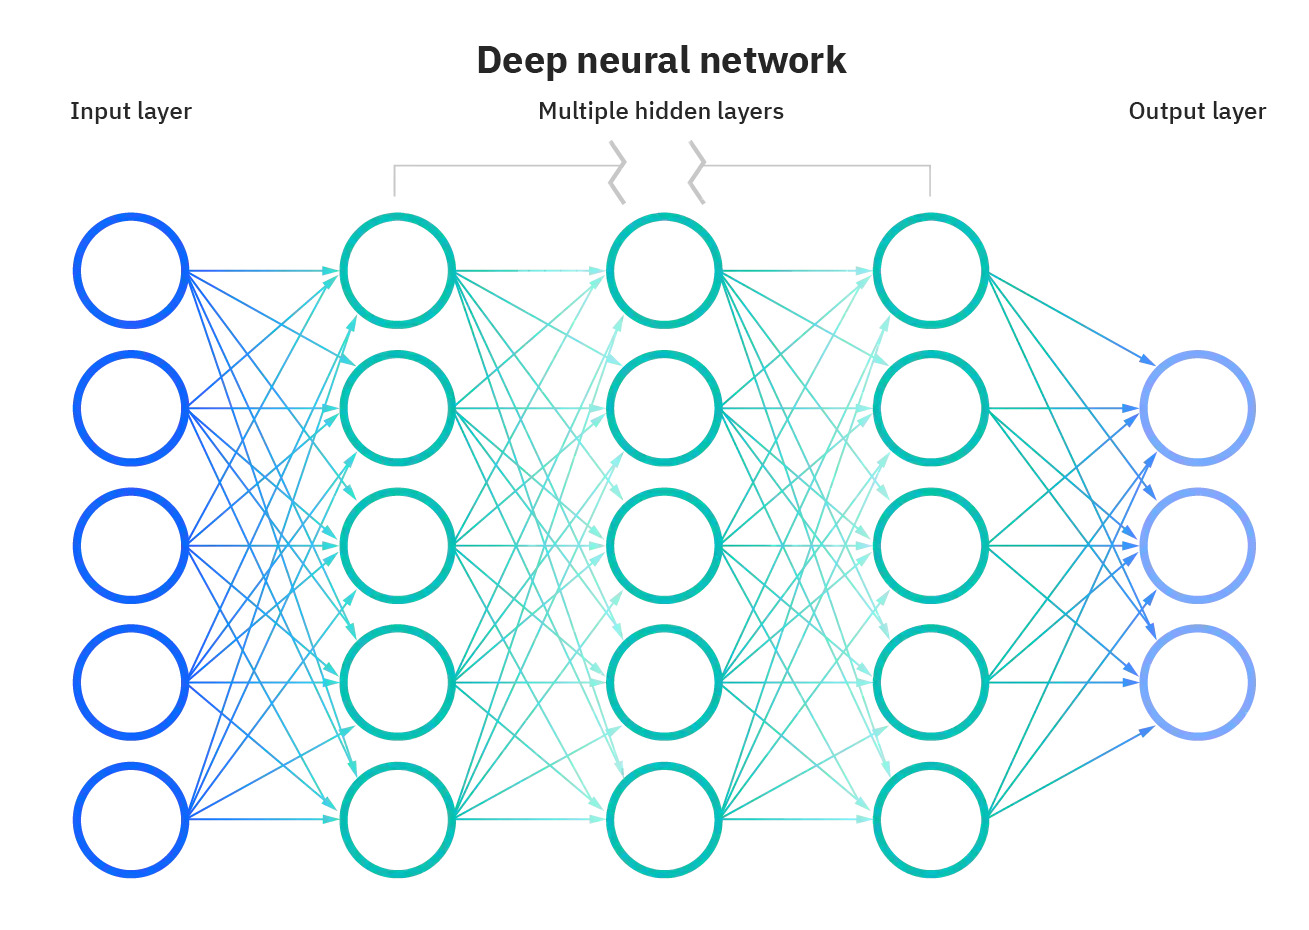
\includegraphics[width=1\textwidth]{pics/neuralnetwork.jpg}
\\
\\
\\
The specific details of how a neural network works can vary depending on its architecture and the type of problem it is being used to solve. But in general, a neural network is able to learn from data by adjusting the strength of the connections between its neurons, these connections being called weights, based on the input it receives. Over time, the network is able to improve its predictions by adjusting these weights in a way that minimizes errors between the network's output and the correct output.

\subsection{Solving Methods}
There are three basic methods for solving problems: search-, knowledge-, and algorithmic methods. Every method involves searching through a space of possible solutions whilst optimizing a pre-defined evaluation function, that can lead to the following "Combinatorial explosion". The methods can range from simplex hill climbing via alpha-beta pruning techniques to knowledge "chunking". 
Example: the chess endgame of king and three pawns versus king and three pawns requires an explicit table of half a billion moves and a run-time of ten quadrillion years to evaluate all possibilities. The success of the CMU "chunker" program which uses chess domain knowledge chunks is that it reduces this run-time to about one minute.

\section{How does face tracking work?}
\setauthor{Romeo Bhuiyan}
Face tracking is a technology that allows a computer or device to identify and monitor the movements of a person's face in real time. This is typically done using a combination of computer vision algorithms and specialized hardware, such as a camera or depth sensor.
\\
\\
To track a face, the system first detects the face in the video feed from the camera or depth sensor. This is typically done using a machine learning algorithm trained to recognize faces in images. Once the face has been detected, the system then uses various techniques to track the movements of the face, such as tracking the position of key facial features (such as the eyes and mouth) over time. This allows the system to accurately follow the face as it moves within the frame, even if it turns or changes orientation.
\\
\\
The resulting data can be used for a variety of purposes, such as enabling facial recognition (to identify who the person is), animating virtual characters, or controlling a user interface.

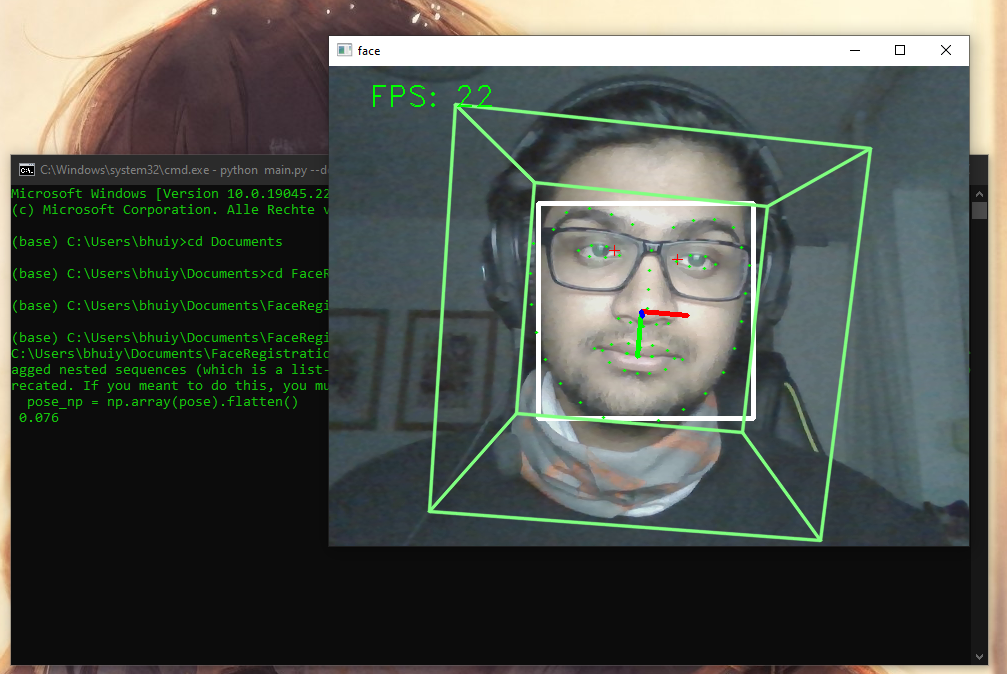
\includegraphics[width=1\textwidth]{pics/bhuiyanfracetracking.png}

% Hier kommt noch unser versuch damit hin

\section{How does body tracking work?}
\setauthor{Romeo Bhuiyan}
Body tracking is the process of using technology to track the movement of a person's body. This is typically done using sensors or cameras that capture the movement of the body and then use algorithms to interpret that movement and translate it into digital data that can be used for various purposes. 
\\
\\
To track a body, the algorithm first detects the presence of a body in the video or data. It then uses various techniques to identify specific features of the body, such as the limbs, torso, or other distinctive features. This allows the algorithm to track the body as it moves over time. 
\\
\\
In addition to tracking the location of the body, some algorithms can also track other features, such as body movements or gestures. This allows them to be used for a variety of applications, such as video surveillance, virtual reality, gaming, human-computer interaction, and fitness tracking.

\section{Performance}
\setauthor{Romeo Bhuiyan}
Performance is important in the field of AI for a number of reasons. Firstly, the goal of AI is to mimic human intelligence and decision-making, for which performance is a key factor in determining how well a machine is able to do this. In order for AI to be useful and effective, it must be able to perform tasks at a level that is comparable to or better than a human.
\\
\\
Performance is also essential due to its determination of speed and efficiency of an AI system. In many cases, the ability of AI to quickly and accurately process large amounts of data and make decisions based on that data can be a key factor in its success. For example, in the field of finance, a high-performing AI system can help traders make faster, more informed decisions, which can lead to better investment returns.
\\
\\
Additionally, it can affect the cost and feasibility of implementing an AI system. If an AI system is not able to perform well, it may be too expensive or too unreliable to be used in practice. As a result, the performance of AI systems is a critical factor that must be considered in the development and deployment of these technologies.
